\documentclass[ruledheader,noindentfirst,anapcustomindent,abntfigtabnum,tocpage=plain]{def_and_cls/abnt}
\usepackage{amsmath, amssymb, amsthm, verbatim, amsfonts, amstext}
%\usepackage[latin1]{inputenc}
\usepackage[brazilian]{babel}
\usepackage[utf8]{inputenc}
\usepackage[T1]{fontenc}
\usepackage{styles/dropping}
\usepackage{graphicx}
\usepackage[hang,small,bf]{caption}
\usepackage[abnt-etal-list=0,abnt-etal-text=it,abnt-and-type=&,abnt-emphasize=bf,abnt-full-initials=yes,alf,bibjustif]{styles/abntcite}
\usepackage{fancyhdr}
\usepackage{makeidx}
\usepackage[none]{hyphenat}
\usepackage{color}
\usepackage{subfig}
\usepackage{styles/algorithms}
\usepackage{algorithmic}
\usepackage{mdwlist}
\usepackage{bm}
\usepackage[titletoc,title]{appendix}
\usepackage{ltxtable}
\usepackage{longtable}
\usepackage{supertabular}
\usepackage{indentfirst}
\usepackage{color}
\usepackage{icomma}

% \usepackage{biblatex} %Imports biblatex package
% \addbibresource{mybibliography.bib} %Import the bibliography file

\usepackage[
    backend=biber,
    style=alphabetic,
    sorting=ynt
]{biblatex}

\addbibresource{bib.bib} %Imports bibliography file

\usepackage[table,xcdraw]{xcolor}

\sloppy


%
%Tradução do pacote Algorithm para portugues
%
\renewcommand{\algorithmicrequire}{\textbf{Entrada:}}
\renewcommand{\algorithmicensure}{\textbf{Saída:}}
\renewcommand{\algorithmicend}{\textbf{fim}}
\renewcommand{\algorithmicif}{\textbf{se}}
\renewcommand{\algorithmicthen}{\textbf{então}}
\renewcommand{\algorithmicelse}{\textbf{senão}}
\renewcommand{\algorithmicelsif}{\algorithmicelse \, \algorithmicif}
\renewcommand{\algorithmicendif}{\algorithmicend \, \algorithmicif}
\renewcommand{\algorithmicfor}{\textbf{para}}
\renewcommand{\algorithmicforall}{\textbf{para todo}}
\renewcommand{\algorithmicdo}{\textbf{fazer}}
\renewcommand{\algorithmicendfor}{\algorithmicend \, \algorithmicfor}
\renewcommand{\algorithmicwhile}{\textbf{enquanto}}
\renewcommand{\algorithmicendwhile}{\algorithmicend \, \algorithmicwhile}
\renewcommand{\algorithmicloop}{\textbf{laço}}
\renewcommand{\algorithmicendloop}{\algorithmicend \, \algorithmicloop}
\renewcommand{\algorithmicrepeat}{\textbf{repetir}}
\renewcommand{\algorithmicuntil}{\textbf{até}}
\renewcommand{\algorithmiccomment}[1]{\{#1\}}
\renewcommand{\listalgorithmname}{Lista de Algoritmos}
\floatname{algorithm}{Algoritmo}
%%%%%%%%%%%%%%%%%%%%%%%%%%%%%%%%%%%%%%%%%%%%%%%%%%%%%%%%%%%%%%%%%%%%%%%%%%%%%%%%%%%

\makeindex

%%%% O arquivo modelosCAP.tex possui as definições para ciação do estilo de capítulo (fonte de título, barras horizontais, etc.)
% ele não gera texto de saída, é um arquivo de configuração somente
%
%Estilo de formatação de capítulos

\makeatletter
\newcommand{\thechapterwords}
{ \ifcase \thechapter\or 1\or 2\or 3\or 4\or 5\or6\or 7\or 8\or 9\or 10\or 11\fi}

\def\@makechapterhead#1{%
\vspace*{10\p@}%
{\parindent \z@  \reset@font

\scshape \@chapapp{} \thechapterwords
\quad %
\par\nobreak
\vspace*{10\p@}%
\interlinepenalty\@M
\hrule
\vspace*{10\p@}%
\Huge \bfseries #1\par\nobreak
\par
\vspace*{10\p@}%
\hrule
\vskip 40\p@
}}
\def\@makeschapterhead#1{%
\vspace*{10\p@}%
{\parindent \z@ \centering \reset@font
\par\nobreak
\vspace*{10\p@}%
\interlinepenalty\@M
\hrule
\vspace*{10\p@}%
\Huge \bfseries #1\par\nobreak
\par
\vspace*{10\p@}%
\hrule
\vskip 40\p@
%\vskip 100\p@
}}
%%%%%%%%%%%%%%%%%%%%%%%%%%%%%%%%%%%%%%%%%%%%%%%FIM DO PREAMBULO%%%%%%%%%%%%%%%%%%%%%%%%%%%%%%%%%%%%%%%%%%%%%%%%%%%%%%%%%%%%%%%%%%


\begin{document}

%%%%% IMPORTANTE: ALTERA O TEXTO ENTRE ARIAL E TIMES NEW ROMAN (ALTERNAR OS COMENTÁRIOS)
%
%%%%%%%%%%%%%%%%%%%%%PARA UTILIZAR ARIAL%%%%%%%%%%%%%%%%%%%%%%%
%
\fontfamily{phv}                    %fonte Arial
\renewcommand{\rmdefault}{phv}      %
%
%%%%%%%%%%%%%%%%%%%%%PARA UTILIZAR TIMES%%%%%%%%%%%%%%%%%%%%%%%
%
%\fontfamily{ptm}               %fonte Times
%\renewcommand{\rmdefault}{ptm} %
%
%%%%%%%%%%%%%%%%%%%%%%%%%%%%%%%%%%%%%%%%%%%%%%%%%%%%%%%%%%%%%%%

%%%%%%%%%%%%%Arquivos .tex com os elementos pré-textuais
%
\thispagestyle{empty}

\vfill
 \begin{center}
    {\large\bfseries ESCOLA POLITÉCNICA DA USP} \\
    \vspace*{1in}
    \begin{figure}[h]
     \centering
            
\includegraphics[width=10cm]{figures/Logo_Poli.jpg}\\
     \end{figure}
    \vspace*{1in}
    \large\bfseries Obtenção e análise de dados referentes à condução de carros
    
    \vspace{1.5cm}
    ANTONIO PINHEIRO DA SILVA JUNIOR - 9004355\\
    ARTHUR PIRES DA FONSECA - 10773096\\
    GABRIEL MORGHETT GABOARDI - 10773968\\
    \vfill
    \large\bfseries{ SÃO PAULO \\ 2023}
\end{center}

\normalsize
\begin{titlepage}
\vfill
\begin{center}
    \vspace{2cm}
    {\Large \textsc{Obtenção e análise de dados referentes à condução de carros}\\}
    \vspace{1cm}
    \hspace{.45\linewidth}
    \begin{minipage}{.50\linewidth}

            Trabalho apresentado à Escola Politécnica da Universidade de São Paulo para
            o Trabalho de Conclusão de Curso em Engenharia de Computação.
            São Paulo
            2020

            \vspace{0.5 cm}

            Orientador:     Prof. Dr. Edson Toshimi Midorikawa\\
            Co-orientador: Prof. Dr. Reginaldo Arakaki\\
    
    \end{minipage}

    \vspace{2cm}
    \vfill
    {\large SÃO PAULO\\ 2022}
\end{center}

\end{titlepage}
\include{3-folhadeaprovacao}
\chapter*{Dedicatória}

\noindent Dedico este trabalho à Hihi e aos meus avós por terem cuidado de mim, ao meu irmão (o Di), e aos meus pais, Alfredo e Márcia.
\chapter*{Agradecimentos}

\noindent Agradecimentos texto.\\

Agradecemos ao Guilherme Migliati https://www.linkedin.com/in/guimigli?utm_source=share&utm_campaign=share_via&utm_content=profile&utm_medium=android_app foram essenciais para superar obstáculos no desenvolvimento do aplicativo, oferecendo suporte técnico, que permitiu a compilação dele.

\\

Além disso, a contribuição significativa do Dr.-Ing. Philippe Jardin https://www.linkedin.com/in/dr-ing-philippe-jardin-964733a3?utm_source=share&utm_campaign=share_via&utm_content=profile&utm_medium=android_app , que disponibilizou o simulador de OBD quando o Arthur ainda estava na Alemanha, ampliou consideravelmente as capacidades de teste do sistema. 

\chapter*{Epígrafe}

\noindent Epígrafe texto.\\
\pagestyle{plain}%%%%% Utilizar ESTILO PLAIN AQUI%%%%%%%
\chapter*{Resumo}

\noindent Este trabalho visa desenvolver a especificação de um sistema 'gimbal' open-source e open-hardware de baixo custo visando tornar esta tecnologia mais acessível. A demanda foi identificada pelo integrante Breno, ao perceber que os fabricantes cobravam preços muito altos inclusive por equipamentos amadores. \\
Especificamos o uso do microcontrolador ATMega328P por ser fácil de obter e estar presente na plataforma Arduino, ao qual a maioria dos usuários tem acesso. O OS escolhido é o armOS, por ter capacidades de tempo real, e que se comunicará com os periféricos: um giroscópio, acelerômetro, botões, servo-motores e LEDs.
\chapter*{Abstract}


\noindent Aiming to create a complementary platform for the driver and his car, this work used different sensors inside a car and those present in a cell phone to build a data compilation platform.\\
Data collection from the car was done through an OBD-II port, present in all vehicles manufactured from 2010 onwards in Brazil. Examples of data collected from a cell phone include information about the car's movement, such as geolocation and acceleration.\\
The collected data, in turn, was passed to the AWS cloud, for profile analysis of each driver.\\
% Each driver will be able to consult their personal data through a system with authentication, which is an exercise of implementation of security, an aspect fundamental to data protection.

%%%Comandos para criação automática das listas
%
\tableofcontents
\listoffigures
\listoftables

%%%Comandos para criar outras listas não suportadas pelo pacote ABNTex%%%
%
\pretextualchapter{Lista de Símbolos}
\begin{basedescript}{\desclabelstyle{\pushlabel}\desclabelwidth{6em}}
\item[$Z$] variavel aleatoria%
\item[$\mathbb{R}$] conjunto dos números reais%
\item[$t$] tempo contínuo%
\item[$n$] tempo discreto%
\item[$f(z)$] função densidade de probabilidade%
\item[$F(z)$] função de distribuição acumulada%
\item[$\sigma$] desvio padrão%
\item[$\mu$] média ou esperança matemática%
\item[$|\cdot|$] operador magnitude%
\item[$\nabla$] operador gradiente%
\end{basedescript}
\newpage

\pretextualchapter{Lista de Abreviacoes}

\begin{basedescript}{\desclabelstyle{\pushlabel}\desclabelwidth{6em}}
% \item[{ANOVA}] \textit{Analysis of Variance}
\item[{API}] \textit{Application Programming Interface}
\item[{AWS}] \textit{Amazon Web Services}
\item[{IDE}] \textit{Integrated Development Environment}
\item[{IoT}] \textit{Internet of Things}
\item[{JSON}] \textit{Java Script Object Notation}
\item[{MVP}] \textit{Minimum Viable Product}
\item[{OBD-II}] \textit{On-board diagnostics}
\item[{PID}] \textit{Parameter Identifier}
\item[{RDS}] \textit{Amazon Relational Database Service}
\item[{RPM}] \textit{Revoluções por minuto}

% \item[{fda}] Função de distribuição acumulada%
% \item[{EMQ}] Erro médio quadrático%
\end{basedescript}
\newpage
%%%%%%%%%%%%%%%%%%%%%%%%%%%%%%%%%%%%%%%%%%%%%%%%%%%%%%%%%%%%%%%%%%%%

%Capítulos passam a ter páginas numeradas
%
\pagestyle{fancy}

%resseta os contadores de capítulo e seção
%
\renewcommand{\chaptermark}[1]{\markboth{#1}{}}
\renewcommand{\sectionmark}[1]{\markright{\thesection\ #1}}

%%%%%%%%%%%%%%NÃO LEMBRO O QUE FAZ, APARENTEMENTE NADA, TESTAR DEPOIS
%\fancyhf{}%
%\fancyhead[RO,LE]{\large\slshape\thepage}%
%\fancyhead[CE]{\large\slshape\leftmark}%
%\fancyhead[CO]{\large\slshape\rightmark}%


%%% Outros arquivos .tex. É acoselhável utilizar vários arquivos, pelo menos um por capítulo
\chapter{Introdução}\label{CAP:introducao}

Este documento consiste de um modelo basico para a producao de documentos academicos, seguindo as normas ABNT. 

Nao e abordado o estudo do LaTex neste template. Sugerimos a leitura do texto em \citeonline{Oetiker:1995}. O uso do LaTex e aconselhavel devido a sua qualidade grafica, facil referenciacao, criacao de listas, indices, referencias bibliograficas e escrita matematica profissional. Porem, nao e obrigatorio o uso deste template, apenas as orientacoes de formatação segundo as normas ABNT devem ser obrigatoriamente seguidas.

Uma observação em particular é a de que, no pacote ABNTex, as referências diretas devem utilizar o comando ``citeonline''. Referências indiretas utilizam o comando ``cite''.

Exemplo de citacao direta: Uma otima fonte de estudo para compreender o LaTex e apresentada por \citeonline{Oetiker:1995}. 

Exemplo de citação indireta: Existem boas fontes de pesquisa para entendimento do LaTex \cite{Oetiker:1995}, estas incluem documentação online disponível na web.

\section{Motivação}

Qual o perfil de direção de um motorista? Como categorizar os condutores segundo um critério claro?

Buscando responder essas perguntas e, consequentemente, entender as características de pessoas ao volante, este trabalho propõe-se a criar uma infraestrutura de captura e análise de dados em automóveis de uso pessoal.

As informações recolhidas serão armazenadas em uma plataforma de nuvem, protegidas por algum nível de segurança, implementado neste mesmo projeto e, por fim, serão analisadas para gerarem conclusões interessantes sobre o modo de dirigir de cada participante do estudo.
	
Uma pesquisa preliminar sobre o assunto revelou que já existe uma patente para um produto parecido; ela foi registrada em 2013 e avalia o desempenho de um motorista a partir de dados pré-coletados de parâmetros relevantes à condução do carro [REFERENCIA 1].

Visão lateral do carro proposto na patente.[IMAGEM, REF 1]

[CITAR OS TRABALHOS QUE JÁ FAZEM ISSO QUE EU DISSE]

\section{Objetivo}

Este trabalho procura analisar o comportamento de motoristas em situações diversas: no trânsito, em uma prova de direção ou em uma rodovia, por exemplo.

Para isso, fará uso da infraestrutura já presente em carros atuais, conforme pode ser visto na imagem a seguir, mas também pode complementá-la com mais equipamentos, caso seja necessário para o projeto.

[IMAGEM]
Sensores estão presentes em um carro atual na ordem de dezenas[2].

A coleta de dados será feita, a princípio, a partir de ensaios em carros reais feitos por uma quantidade seleta de pessoas, que pode ser expandida para resultados mais precisos na análise posterior.

Os dados coletados deverão ser passados para algum serviço de nuvem, usando conexão à Internet, caracterizando uma aplicação IoT.
	
Do lado da nuvem, será possível utilizar os dados de cada usuário de forma anônima, para diagnosticar o perfil do condutor e possivelmente gerar insights sobre como a pessoa poderia melhorar.
	
A plataforma poderá, após implementada, servir como base de dados para outros projetos futuros, que não farão parte deste TCC, por exemplo:

Prova de direção usando Inteligência Artificial: possível supressão da prova do Detran, avaliando o condutor ao longo das aulas práticas

Seguros de carro personalizados: valores mais altos para motoristas mais violentos

Classificação de motoristas de aplicativo: avaliação ponderada pela forma de dirigir

 
\section{Justificativa}
ROMEO e PIRES [GIT]
Pq o trabalho é importante?


\section{Organização do trabalho}
[ANTIGO "PROCUCAO CIENTIFICA"]

O padrão OBD-II foi uma extensão do padrão OBD-I, uniformizando esse tipo de conector em casos em geral, começando a ser adotado no Brasil a partir de 2010[4].

Nesse padrão de conexão e comunicação é definida uma interface por onde parâmetros internos a um carro podem ser monitorados.

As mensagens definidas pelo OBD-II têm cada uma um PID (parameter ID). O conjunto comum de PIDs de serviços que podem ser solicitados pela porta OBD-II e para que servem pode ser visto na tabela a seguir[REF 3].

[TABELA]

Service / Mode (hex)
Description
01
Show current data - I/M Monitors and Live Data
02
Show Freeze Frame (FF) Data
03
Show Stored Diagnostic Trouble Codes
04
Clear/Erase Diagnostic Trouble Codes and stored values
05
Test results, oxygen sensor monitoring (non CAN only)
06
Test results, other component/system monitoring (Test results, oxygen sensor monitoring for CAN only)
07
Show pending Diagnostic Trouble Codes (detected during current or last driving cycle)
08
Control operation of on-board component/system (EVAP)
09
Request Vehicle Information (VIN)
0A
Permanent Diagnostic Trouble Codes (DTCs) (Cleared DTCs)

É importante notar que os serviços do padrão OBD-II comuns a todos os carros sempre começam com o dígito zero (hexadecimal), por isso, serviços específicos de cada fabricante devem começam a partir do código 0x10.

[IMAGEM]

Posição da porta OBD-II em um carro[5].

Os dados que podem ser coletados de qualquer carros são explicitados na tabela abaixo[3]:

[TABELA]

Interessante notar que, embora não esteja representado na tabela, os PIDs 0x00, 0x20, 0x40, etc, ou seja, a cada 32 valores de PID, existe um parâmetro apenas para indicar quais entre os PIDs seguintes são fornecidos por aquele carro.

Esses PIDs de marcação, por assim dizer, utilizam 4 bytes para comunicar quais dos próximos PIDs estão disponíveis, utilizando cada bit como uma flag binária. 

Na imagem a seguir é possível visualizar como esse processo é feito, usando como exemplo o valor 0xBE1FA813 para representar os 4 bytes oferecidos[3].

[IMAGEM]


\section{Organização da tese}

\noindent \textbf{Capitulo \ref{CAP2}}: descricao...

\noindent \textbf{Capitulo \ref{CAP3}}: descricaoo...

\noindent \textbf{Capitulo \ref{CAP4}}: descricao...

\noindent \textbf{Capitulo \ref{CAP5}}: descricao...
\chapter{Aspectos conceituais}
\label{CAP2}

A seguir serão explicados os conceitos fundamentais que possibilitam a execução deste trabalho. 

% apresentar conceitos empregados e revisao da literatura (parte toerica do trab)

\section{O padrão OBD-II}

Criado na década de 1990 para gerar controle sobre as emissões de gás carbônico dos carros\textsuperscript{[5]}, hoje define um protocolo padronizado para comunicar parâmetros internos do veículo.
    
O padrão OBD-II foi uma extensão do padrão OBD-I, uniformizando esse tipo de conector em casos em geral, começando a ser adotado no Brasil a partir de 2010\textsuperscript{[4]}.

A comunicação é feita através de uma conexão física que normalmente pode ser encontrada abaixo do volante do motorista\textsuperscript{[5]}, conforme indicado pela figura \ref{fig:obd2_conn}.

Nesse padrão de conexão e comunicação é definida uma interface por onde parâmetros internos a um carro podem ser monitorados.

As mensagens definidas pelo OBD-II têm cada uma um PID (\textit{Parameter ID}). O conjunto comum de PIDs de serviços que podem ser solicitados pela porta OBD-II e para que servem pode ser visto na tabela \ref{Tb:tab1}\textsuperscript{[3]}.

\begin{table}[]
% \begin{adjustbox}{width=\textwidth}
\begin{tabular}{cc}
\rowcolor[HTML]{656565} 
{\color[HTML]{FFFFFF} Service / Mode (hex)} & {\color[HTML]{FFFFFF} Description}                                                                    \\
01                                          & Show current data - I/M Monitors and Live Data                                                        \\
02                                          & Show Freeze Frame (FF) Data                                                                           \\
03                                          & Show Stored Diagnostic Trouble Codes                                                                  \\
04                                          & Clear/Erase Diagnostic Trouble Codes and stored values                                                \\
05                                          & Test results, oxygen sensor monitoring (non CAN only)                                                 \\
06                                           & Test results, other component/system monitoring (Test results, oxygen sensor monitoring for CAN only) \\
07                                           & Show pending Diagnostic Trouble Codes (detected during current or last driving cycle)                 \\
08                                           & Control operation of on-board component/system (EVAP)                                                 \\
09                                          & Request Vehicle Information (VIN)                                                                     \\
0A                                          & Permanent Diagnostic Trouble Codes (DTCs) (Cleared DTCs)                                             
\end{tabular}
\end{table}

É importante notar que os serviços do padrão OBD-II comuns a todos os carros sempre começam com o dígito zero (hexadecimal), por isso, serviços específicos de cada fabricante devem começam a partir do código 0x10.

\begin{figure}[hp]
    \centering
    
    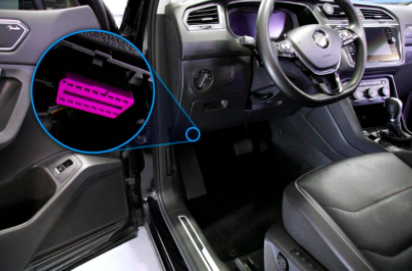
\includegraphics[]{figures/localizacao_obd2.png}
    
    \caption{Posição da porta OBD-II em um carro\textsuperscript{[5]}}
    
    \label{fig:obd2_conn}
\end{figure}

Os dados que podem ser coletados de qualquer carro são explicitados na tabela \ref{Tb:tab2}\textsuperscript{[3]}.

% Please add the following required packages to your document preamble:
% \usepackage[table,xcdraw]{xcolor}
% If you use beamer only pass "xcolor=table" option, i.e. \documentclass[xcolor=table]{beamer}
\begin{table}[]
\begin{tabular}{ccccccc}
\rowcolor[HTML]{C0C0C0} 
{\color[HTML]{FFFFFF} \textbf{PIDs(hex)}} & {\color[HTML]{FFFFFF} \textbf{PID(Dec)}} & {\color[HTML]{FFFFFF} \textbf{Data bytes returned}} & {\color[HTML]{FFFFFF} \textbf{Description}} & {\color[HTML]{FFFFFF} \textbf{Min value}} & {\color[HTML]{FFFFFF} \textbf{Max value}} & {\color[HTML]{FFFFFF} \textbf{Units}} \\
04                                         & 4                                        & 1                                                   & Calculated engine load                      & 0                                         & 100                                       & \%                                    \\
0C                                        & 12                                       & 2                                                   & Engine speed                                & 0                                         & 16,383.75                                 & rpm                                   \\
0D                                        & 13                                       & 1                                                   & Vehicle speed                               & 0                                         & 255                                       & km/h                                  \\
0F                                        & 15                                       & 1                                                   & Intake air temperature                      & -40                                       & 215                                       & °C                                    \\
1F                                        & 31                                       & 2                                                   & Run time since engine start                 & 0                                         & 65,535                                    & seconds                               \\
33                                        & 51                                       & 1                                                   & Absolute Barometric Pressure                & 0                                         & 255                                       & kPa                                   \\
46                                        & 70                                       & 1                                                   & Ambient air temperature                     & -40                                       & 215                                       & °C                                    \\
47                                        & 71                                       & 1                                                   & Absolute throttle position B                & 0                                         & 100                                       & \%                                    \\
49                                        & 73                                       & 1                                                   & Accelerator pedal position D                & 0                                         & 100                                       & \%                                    \\
51                                        & 81                                       & 1                                                   & Fuel Type                                   & -                                         & -                                         & -                                     \\
52                                        & 82                                       & 1                                                   & Ethanol fuel \%                             & 0                                         & 100                                       & \%                                    \\
5A                                        & 90                                       & 1                                                   & Relative accelerator pedal position         & 0                                         & 100                                       & \%                                    \\
5B                                        & 91                                       & 1                                                   & Hybrid battery pack remaining life          & 0                                         & 100                                       & \%                                    \\
5C                                        & 92                                       & 1                                                   & Engine oil temperature                      & -40                                       & 210                                       & °C                                    \\
5D                                        & 93                                       & 2                                                   & Fuel injection timing                       & -210.00                                   & 301992                                    & °                                     \\
5E                                        & 94                                       & 2                                                   & Engine fuel rate                            & 0                                         & 3212.75                                   & L/h                                   \\
61                                        & 97                                       & 1                                                   & Driver's demand engine - percent torque     & -125                                      & 130                                       & \%                                    \\
62                                        & 98                                       & 1                                                   & Actual engine - percent torque              & -125                                      & 130                                       & \%                                    \\
63                                        & 99                                       & 2                                                   & Engine reference torque                     & 0                                         & 65,535                                    & Nm                                    \\
64                                        & 100                                      & 5                                                   & Engine percent torque data                  & -125                                      & 130                                       & \%                                    \\
70                                        & 112                                      & 10                                                  & Boost pressure control                      & -                                         & -                                         & -                                     \\
83                                        & 131                                      & 9                                                   & NOx sensor                                  & -                                         & -                                         & -                                     \\
8E                                        & 142                                      & 1                                                   & Engine Friction - Percent Torque            & -125                                      & 130                                       & \%                                   
\end{tabular}
\end{table}

Interessante notar que, embora não esteja representado na tabela, os PIDs 0x00, 0x20, 0x40, etc, ou seja, a cada 32 valores de PID, existe um parâmetro apenas para indicar quais entre os PIDs seguintes são fornecidos por aquele carro.

Esses PIDs de marcação, por assim dizer, utilizam 4 bytes para comunicar quais dos próximos PIDs estão disponíveis, utilizando cada bit como uma \textit{flag} binária. 

Na figura \ref{fig:bitwise_obd2} é possível visualizar como esse processo é feito, usando como exemplo o valor \textit{0xBE1FA813} para representar os 4 bytes oferecidos\textsuperscript{[3]}.

\begin{figure}[hp]
    \centering
    
    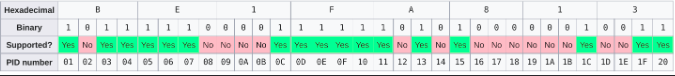
\includegraphics[scale=0.7]{figures/tabela_dados_disponiveis.png}
    
    \caption{Divisão bit a bit da mensagem OBD-II informando os serviços disponíveis\textsuperscript{[3]}}
    
    \label{fig:bitwise_obd2}
\end{figure}

A coleta de fato dos dados relevantes será feita por uma aplicação desenvolvida \textit{a priori} que já é capaz de comunicar-se corretamente com a interface OBD.

Essa aplicação acelerará a criação da infraestrutura proposta por este trabalho, uma vez que pula o primeiro passo da estratégia \textit{bottom-up} que deverá permear o projeto.

\section{Transmissão de dados}

A implementação da transmissão \textit{Bluetooth} neste projeto de compilação de dados oferece uma solução eficaz para a comunicação entre os produtor e consumidor de dados. 

Ao utilizar essa tecnologia, os dados de rastreamento podem ser transmitidos de forma sem fio e em tempo real para dispositivos equipados com \textit{Bluetooth}, como \textit{smartphones}, que são o foco deste trabalho.

A abordagem \textit{wireless} proporciona uma conectividade mais flexível, eliminando a necessidade de cabos físicos e simplificando a integração do sistema. A baixa energia do \textit{Bluetooth} permite uma transmissão eficiente de dados, minimizando o impacto no consumo de bateria dos dispositivos móveis.

Além disso, a transmissão \textit{Bluetooth} possibilita a interação direta entre o sistema de geração e os usuários, permitindo a visualização em tempo real de informações de condução.

Essa integração sem fio não apenas aprimora a experiência do usuário, mas também amplia as possibilidades de interatividade e controle, tornando o sistema mais acessível e fácil de usar.

 \begin{figure}[hp]
    \centering
    
    
\includegraphics[scale=0.4]{figures/bluetooth.png}
    
    \caption{Logo do Bluetooth.}
    
\end{figure}

\section{Armazenamento em nuvem}
Provedoras como a Amazon e a Azure (Microsoft) oferecem serviços de nuvem que podem ser usados para este projeto \textsuperscript{[10, 11]}. Neste trabalho, optou-se pelo serviço da AWS, uma vez que um dos integrantes do grupo já tinha familiaridade com o serviço.

A integração do aplicativo Android com o Amazon RDS (Relational Database Service) da AWS oferece uma solução eficiente e escalável para o armazenamento de dados. 

Utilizando o RDS, os dados coletados, como informações de localização, velocidade e aceleração, podem ser armazenados em bancos de dados relacionais, proporcionando alta disponibilidade, segurança e desempenho otimizado. 

A flexibilidade do Amazon RDS permite a escolha de diferentes motores de banco de dados, como MySQL, PostgreSQL, ou SQL Server, adequando-se às necessidades específicas do sistema.

Os usuários poderão transmitir informações para a nuvem a qualquer momento, desde que seus carros estejam ligados e conectados à internet. O volume de dados recebidos no sistema é, portanto, variável e por isso fez sentido que o serviço de nuvem contratado siga o modelo \textit{on-demand}. A figura \ref{figure:custo_aws_inicial} mostra o custo calculado no serviço da AWS RDS.

\begin{figure}[hp]
    \centering
    
    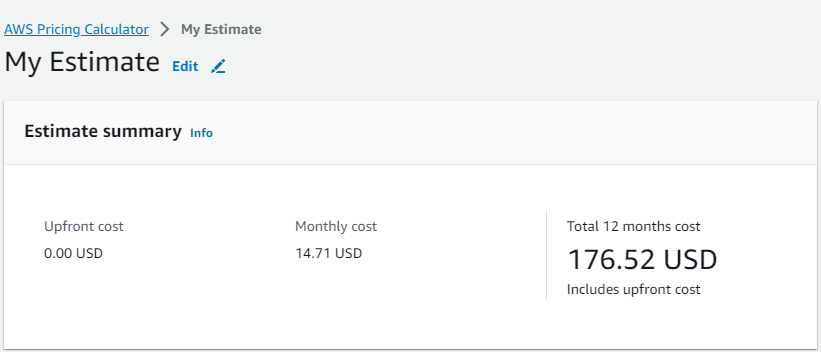
\includegraphics[scale=0.8]{figures/custo_aws_inicial.PNG}
    \caption{Custo da AWS.}
    \label{figure:custo_aws_inicial}
    
\end{figure}

A região do Leste da Virgina é conhecida por ter uma alta densidade de \textit{data centers}. Isso resulta em eficiência operacional e redução de custos.

A instância escolhida foi a \textbf{db.t3.micro}. Ela é uma instância de banco de dados pequena, sendo adequada para cargas de trabalho leves. Essa instância é comumente usada para ambientes de desenvolvimento, testes ou pequenas aplicações que não exigem muitos recursos.

Um RDS Proxy é um serviço que facilita a escalabilidade e a alta disponibilidade para as conexões de banco de dados. Ele ajuda a melhorar o desempenho e a segurança ao gerenciar as conexões entre seus aplicativos e instâncias de banco de dados RDS. Isso é especialmente útil em ambientes onde há flutuações na carga de trabalho. Como se trata de um protótipo, não há preocupações com carga de trabalho. Logo, essa opção não foi escolhida.

Também não há necessidade de ter um ambiente de zona de disponibilidade múltipla para garantir escalabilidade, pois haveria custo adicional. Por isso, a instância RDS foi configurada para o modo Single-AZ. E a capacidade de armazenamento foi 20 GB.


\begin{table}[]
\begin{tabular}{|ll|}
\hline
\multicolumn{1}{|l|}{\textbf{Região}}                 & Virgínia     \\ \hline
\multicolumn{1}{|l|}{}                                &              \\ \hline
\multicolumn{2}{|c|}{\textbf{Especificação das instancias do MySQL}} \\ \hline
\multicolumn{1}{|l|}{Quantidade de Instancias MYSQL}  & 1            \\ \hline
\multicolumn{1}{|l|}{tipo da instancia}               & db.t3.micro  \\ \hline
\multicolumn{1}{|l|}{vCPU}                            & 2            \\ \hline
\multicolumn{1}{|l|}{Memória}                         & 1GiB         \\ \hline
\end{tabular}
\end{table}
\chapter{Metodologia do trabalho / tecnologias utilizadas}
\label{CAP3}

Esta seção trata das fases do trabalho: como deverão ser executadas e em que sequência.

% descrever fases do trab: concepcao, projeto, implementacao, testes
% (falar com o prof)


\section{OBD-II / coleta dos dados}
A plataforma aceleradora desenvolvida no GitHub[REF 12] deverá comunicar-se com o veículo através do protocolo OBD-II.

Esta fase do desenvolvimento caracteriza-se pela adaptação do aplicativo para que possa atender aos requisitos do projeto.

Primeiro, será preciso entender a estrutura e o funcionamento do código através da IDE do \textit{Android Studio}, que foi por onde essa plataforma foi originalmente desenvolvida.

Complementarmente ao que for fornecido pela porta OBD, poderão ser usados também dados externos ao carro, como os de navegação fornecidos pelo Waze através dos próprios motoristas que passam em cada via [REF 13], informações de localização via GPS e também a aceleração desempenhada pelo carro durante seu trajeto.

Essas outras informações serão de grande importância na fase final do projeto, de análise dos dados coletados.

\section{Transferência de dados para a nuvem e estruturação}
Uma vez que a plataforma aceleradora esteja adaptada ao novo sistema, os dados coletados deverão ser passados para uma plataforma remota, que armazenará os dados brutos coletados para depois serem processados e analisados na fase seguinte.

O \textit{pipeline} de captura e armazenamento de informações estará consolidado quando for definida uma estrutura fixa para o processamento dos dados crus e o formato em que serão guardados na nuvem.

Isso poderá ser feito fixando-se uma especificação básica de arquivos JSON que deverá ser seguida pelas APIs que fizerem uso do banco de dados da nuvem.

\section{Geração dos dados}
O sistema poderá ser usado assim que os protocolos e estruturas básicos de comunicação tiverem sido definidos. 

Neste momento serão necessários voluntários para fornecer dados ao sistema e quanto mais pessoas puderem participar, melhor será a análise de perfil feita ao fim do projeto.

\section{Visualização dos dados}
Uma aplicação Web básica para visualização dos dados individuais de cada motorista deverá ser implementada.

Essa plataforma deverá permitir que apenas usuários autorizados acessem suas próprias informações. Para isso, algum sistema de segurança deverá ser implementado.

Na área logada do motorista, será possível visualizar estatísticas básicas acerca do que foi coletado pela porta OBD.

A princípio, serão apresentados bem poucos dados, os quais serão definidos assim que o sistema for um pouco mais palpável. 

\section{Análise dos dados}
Finalmente, com toda a infraestrutura do projeto já funcional, será possível gerar estatísticas relevantes sobre cada motorista.

Quais parâmetros serão gerados ou que análise será feita objetivamente ainda será objeto de discussão no projeto, mas uma das ideias primárias era tentar definir métricas que diferenciem um motorista do outro, isto é, que definam o seu perfil de condução.
\chapter{Especificação de requisitos do trabalho}

\label{CAP4}


definir tecnicnas, processos e sistemas, procedimentos que vão compor o sistema


\section{bbbbbbbbbb}



\chapter{Desenvolvimento do trabalho}]

\label{CAP5}


Este capítulo tem como objetivo 


\section{Tecnologias utilizadas???? (nao é aqui) talvez Estrutura}
interface com usuario, banco de dados, conexão obd2

\section{Projeto e implementação}
decisoes feitas durante o trab

\section{Testes e avaliação}
descrever o plano de testes do sistema: testes de software, modulo, integração e validação

Using \texttt{biblatex} you can display a bibliography divided into sections, depending on citation type. 
Let's cite! Einstein's journal paper \cite{einstein} and Dirac's book \cite{dirac} are physics-related items. 
Next, \textit{The \LaTeX\ Companion} book \cite{latexcompanion}, Donald Knuth's website \cite{knuthwebsite}, \textit{The Comprehensive Tex Archive Network} (CTAN) \cite{ctan} are \LaTeX-related items; but the others, Donald Knuth's items, \cite{knuth-fa,knuth-acp} are dedicated to programming. 


\chapter{Interfaces}]

\label{CAP6}


Este capítulo tem como objetivo 


\section{dddddddd}\label{Sub:equa}
SPI (GPIO das placas feitas pela Arduino):
Giroscópio: dados posicionais
Acelerômetro: dados posicionais
Botões (ao menos dois): interface com o usuário
LED (depuração): interface com o usuário
USB:
Carregamento: fazer o código rodar no Arduino 
Depuração: do código na placa

\chapter{Ambiente de desenvolvimento e depuração}]

\label{CAP7}


Este capítulo tem como objetivo 


\section{eeeeeeeeeeeeeeeeee}\label{Sub:equa}

Usaremos as bibliotecas de cada sensor e motor a ser usado, para facilitar a integração
Não há necessidade de sistema de arquivos, já que os dados são tratados ativamente
Usaremos os drivers de interface com o GPIO fornecidos pelo SO
A depuração será feita em cada camada de maneiras diferentes: 
Simulação → aplicação 
QEMU → SO 
LEDs → hardware 

\chapter{Apêndices}\label{CAP:integracao}

\label{CAP8}

Como juntar todas as subpartes do projeto é uma outra tarefaimportante de engenharia.

A seguir é descrito como isso pode ser feito.

\section{Compra da placa ATMEGA}
\section{Compra da placa ATMEGA}
\section{Compra da placa ATMEGA}
\section{Compra da placa ATMEGA}
\section{Compra da placa ATMEGA}
\chapter{Anexos}]

\label{CAP9}


Este capítulo tem como objetivo 


\section{eeeeeeeeeeeeeeeeee}\label{Sub:equa}

Usaremos as bibliotecas de cada sensor e motor a ser usado, para facilitar a integração
Não há necessidade de sistema de arquivos, já que os dados são tratados ativamente
Usaremos os drivers de interface com o GPIO fornecidos pelo SO
A depuração será feita em cada camada de maneiras diferentes: 
Simulação → aplicação 
QEMU → SO 
LEDs → hardware 


%%%% Estilo de citação ABNT e arquivo de bibitens (mybibliography.bib)
% \bibliographystyle{abnt-alf}
% \bibliography{mybibliography}
% \printbibliography


\chapter{Referências}

[1] “US20130052614A1 - Driver Performance Metric.” Google Patents, Google, disponível em <patents.google.com/patent/US20130052614>. Acesso em 30 de janeiro de 2022

[2] Paulo Campo Grande. “Novas Tecnologias: Carros Atuais Têm Até 100 Sensores a Bordo.” Quatro Rodas, 12 de junho de 2018, disponível em <quatrorodas.abril.com.br/noticias/novas-tecnologias-carros-atuais-tem-ate-100-sensores-a-bordo/>. Acesso em 20 de fevereiro de 2022

[3] “OBD-II PIDs.” Wikipedia, Wikimedia Foundation, 17 Mar. 2022, disponível em <en.wikipedia.org/wiki/OBD-II_PIDs>. Acesso em 20 de março de 2022

[4] Sobre o autor Nina Finco Formada em jornalismo pela UMESP-SP e especialista em mídia. “OBD: o Que é e Para Que Serve o Protocolo OBD2?” Blog Da Cobli, 9 Sept. 2021, disponível em <www.cobli.co/blog/o-que-e-protocolo-obd2/>. Acesso em 20 de março de 2022

[5] “What Is OBDII? History of on-Board Diagnostics.” Geotab, disponível em <www.geotab.com/blog/obd-ii/>. Acessado em 20 de março de 2022

[6] https://www.sbtnews.com.br/noticia/brasil/194388-no-brasil--cerca-de-32-pessoas-morrem-por-dia-em-acidentes-de-transito#:~:text=Em%202021%2C%20foram%2011.647%20mortes,incidentes%20por%20hora%20no%20Brasil.

[7] https://news.un.org/pt/story/2021/11/1771092

[8] https://ourworldindata.org/grapher/covid-deaths-income, consultado em 18 de abril de 2022

[9] https://www.jaguarbrasil.com.br/news/em-quanto-tempo-os-carros-autonomos-serao-o-novo-padrao.html#:~:text=A%20ind%C3%BAstria%20de%20pesquisa%20IHS,pode%20demorar%20um%20pouco%20mais.



\newpage
% \referencias
\bibliography{bib/bib.bib}


% \printbibliography[
%     heading=bibintoc,
%     title={Referências}
% ] %Prints the entire bibliography with the title "Whole bibliography"

% \apendice
% \include{appendices}




\end{document}